\begin{figure*}[hbtp]
  \centering
  % \includegraphics[width=0.44\linewidth]{out/insertions-error-key.pdf}
  \subfigure[Overall result]{
    \label{fig:insertions-error--mean}
    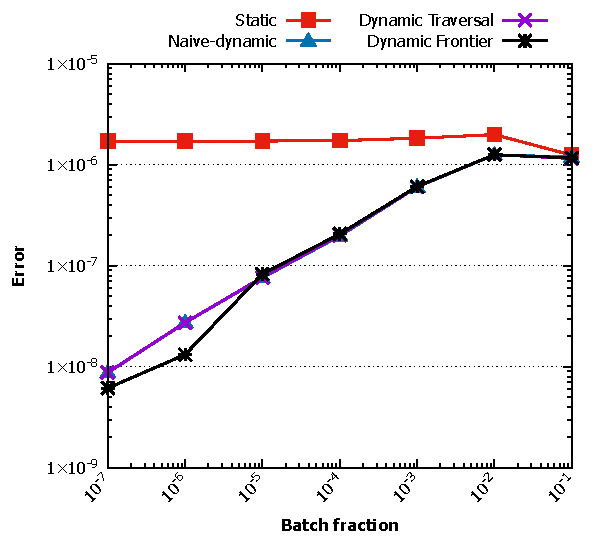
\includegraphics[width=0.38\linewidth]{out/insertions-error-mean.pdf}
  }
  \subfigure[Results on each graph]{
    \label{fig:insertions-error--all}
    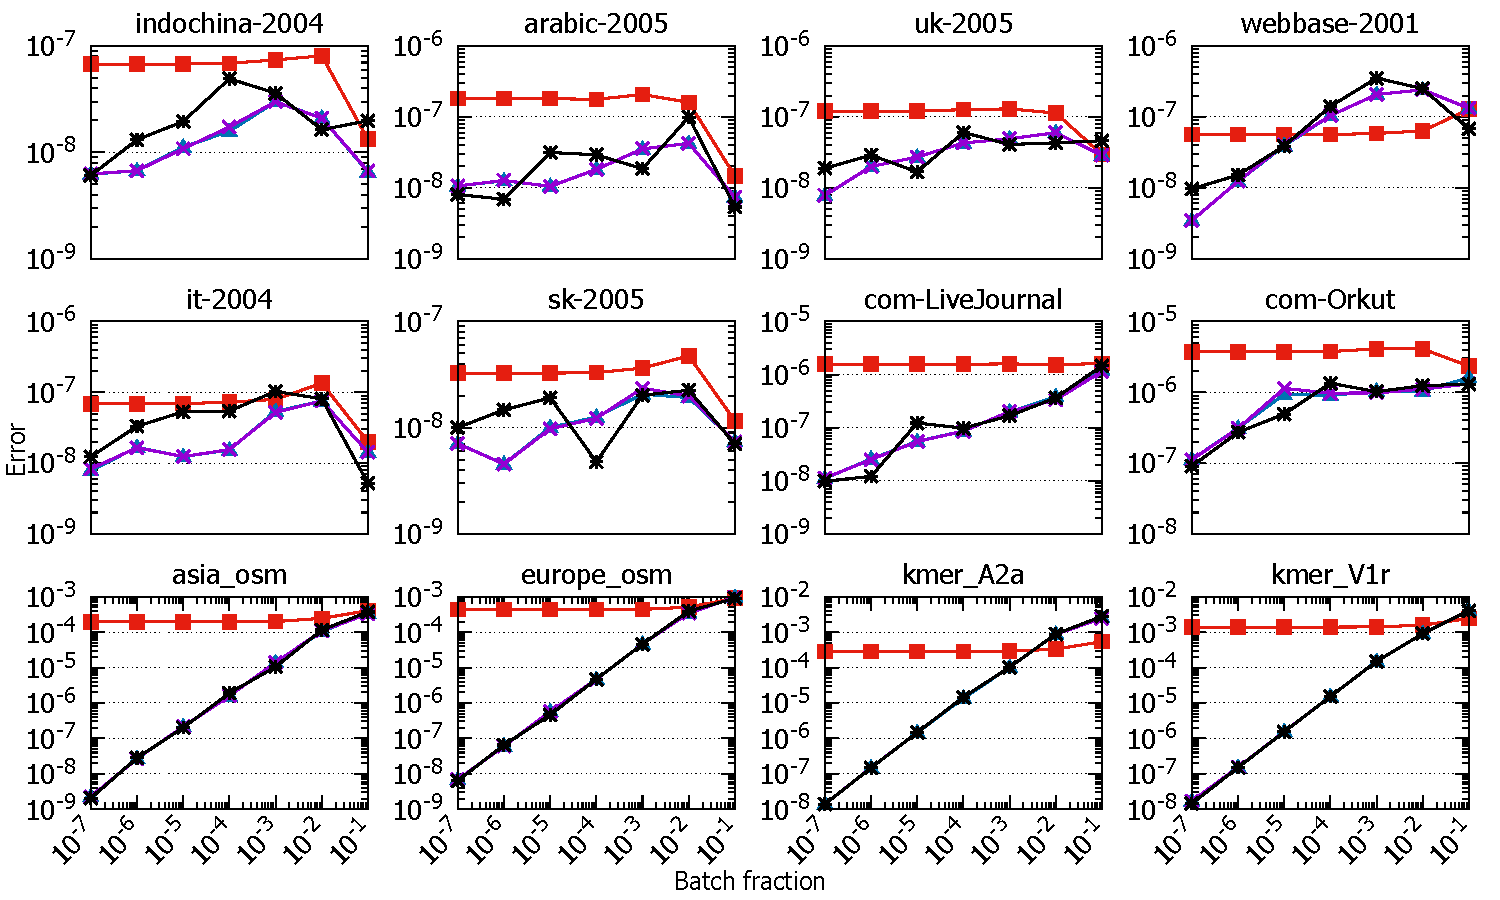
\includegraphics[width=0.58\linewidth]{out/insertions-error-all.pdf}
  } \\[-1ex]
  \caption{Error analysis comparing \textit{Static}, \textit{Naive-dynamic}, \textit{Dynamic Traversal}, and \textit{Dynamic Frontier} PageRank with a Reference Static PageRank (with a tolerance $\tau$ of $10^{-100}$ and limited to $500$ iterations) using $L1$-norm. Batch updates involve edge insertions ranging from $10^{-7} |E|$ to $0.1 |E|$ (logarithmic scale). The right figure illustrates the error specific to each approach for individual graphs in the dataset, while the left figure presents overall errors using the geometric mean for consistent scaling across graphs.}
  \label{fig:insertions-error}
\end{figure*}
